\documentclass[12pt]{letter}\usepackage[letterpaper,margin=0.65in]{geometry}\usepackage{textcomp}\usepackage{graphicx}\usepackage[rflt]{floatflt}\pagenumbering{gobble}\begin{document}\begin{floatingfigure}{0.15\textwidth}\raisebox{0pt}[0pt][0pt]{\raisebox{-2.5cm}{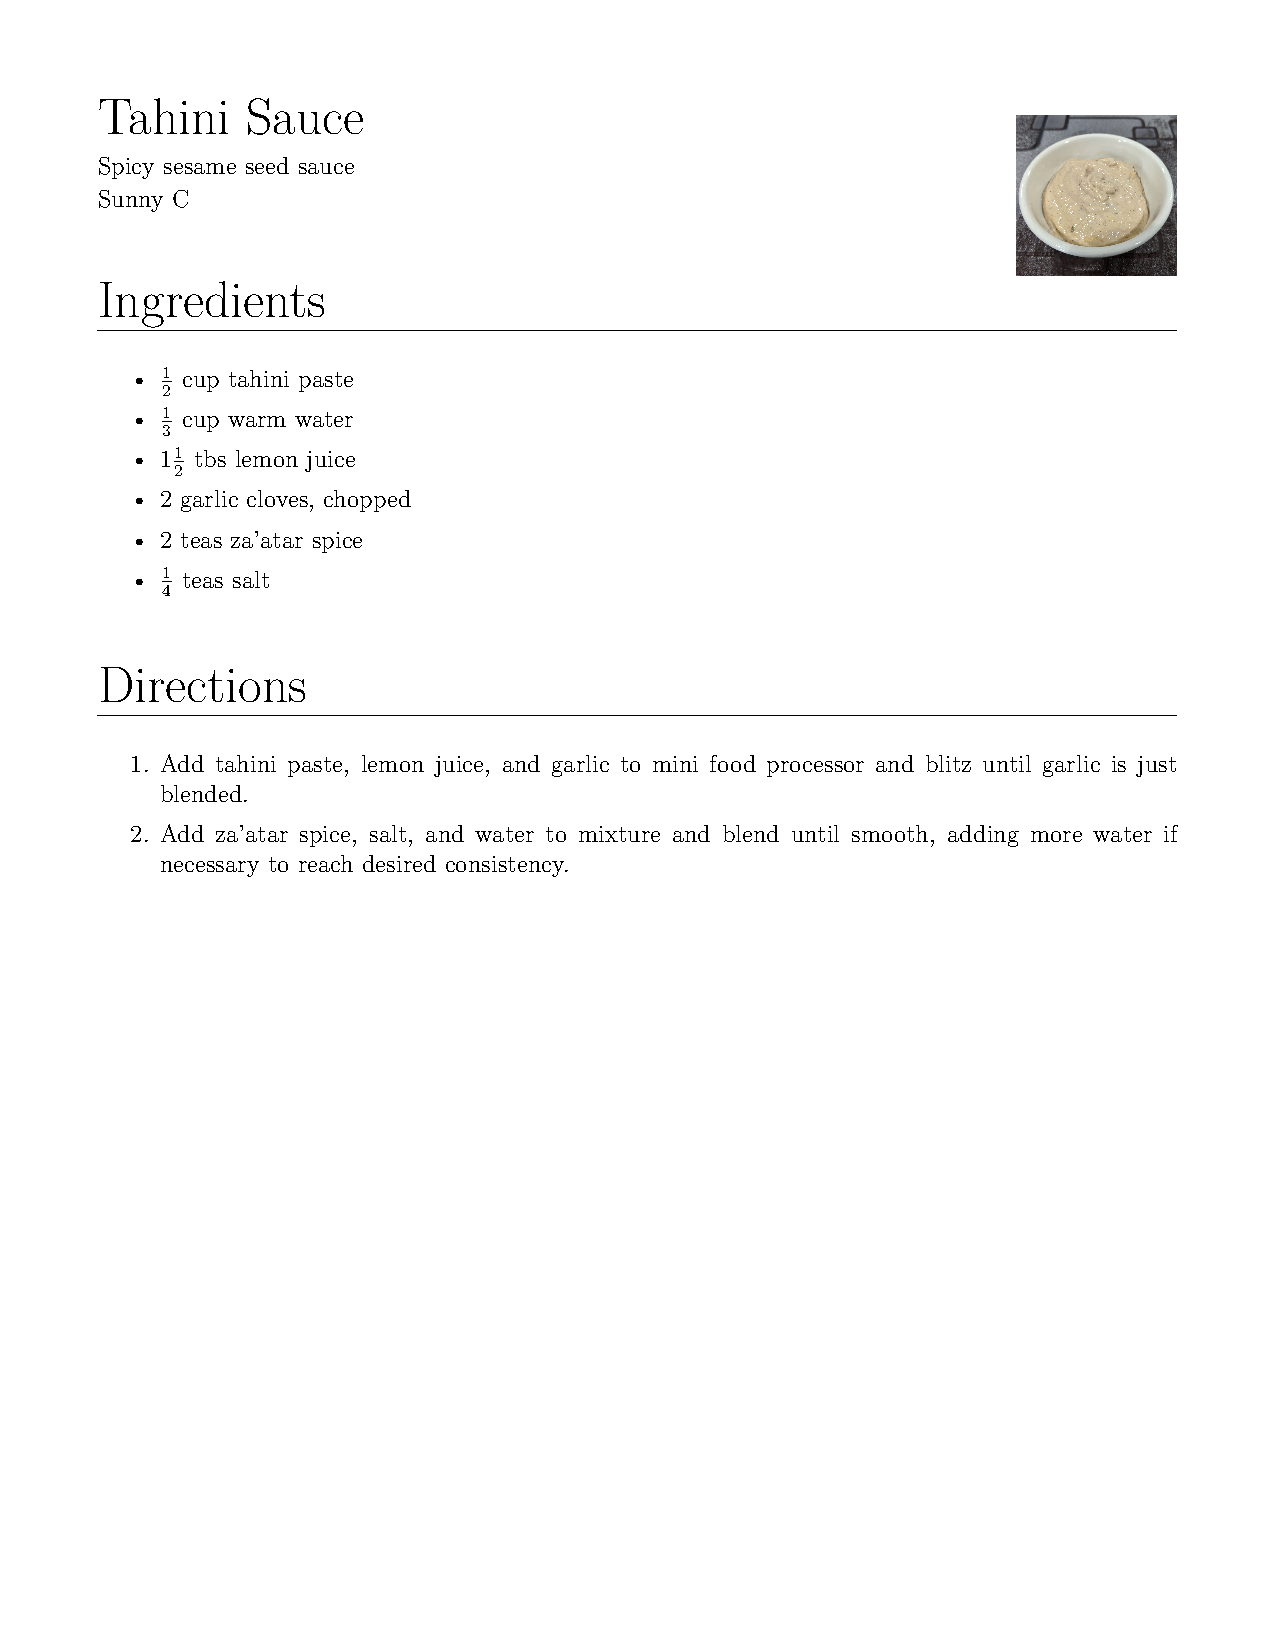
\includegraphics[width=0.15\textwidth]{tahini-sauce}}}\end{floatingfigure}\begin{huge}Tahini Sauce\end{huge}\newline\vspace{-2.5mm}\newline\renewcommand{\arraystretch}{1.1}\begin{tabular*}{\textwidth}{@{\extracolsep{\fill}}lr}Spicy sesame seed sauce\\Sunny C\end{tabular*}\newline\vspace{10mm}\newline\begin{huge}Ingredients\end{huge}\\\rule[2.8mm]{\textwidth}{.1pt}\vspace{-3mm}\begin{itemize}\item $\frac{1}{2}$ cup tahini paste\item $\frac{1}{3}$  cup warm water\item 1$\frac{1}{2}$ tbs lemon juice\item 2 garlic cloves, chopped\item 2 teas za'atar spice\item $\frac{1}{4}$ teas salt\end{itemize}\vspace{7mm}\begin{huge}Directions\end{huge}\\\rule[2.8mm]{\textwidth}{.1pt}\vspace{-3mm}\begin{enumerate}\item Add tahini paste, lemon juice, and garlic to mini food processor and blitz until garlic is just blended.\item Add za'atar spice, salt, and water to mixture and blend until smooth, adding more water if necessary to reach desired consistency.\end{enumerate}\end{document}